\paragraph{QuizziPedia::Front-End::Controllers::FillingQuestionnaireController}
\begin{figure} [ht]
	\centering
	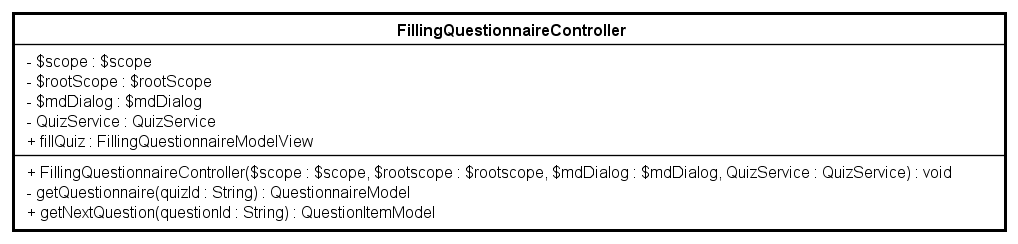
\includegraphics[scale=0.45]{UML/Classi/Front-End/QuizziPedia_Front-end_Controller_FillingQuestionnaireController.png}
	\caption{QuizziPedia::Front-End::Controllers::FillingQuestionnaireController}
\end{figure} \FloatBarrier
\begin{itemize}
	\item \textbf{Descrizione}: questa classe permette di gestire la compilazione del questionario;
	\item \textbf{Utilizzo}: fornisce le funzionalità per compilare un questionario e per gestire il cambio di domanda;
	\item \textbf{Relazione con altre classi}:
	\begin{itemize}
		\item \textit{IN} \texttt{FillingQuestionnaireModelView}: ;  
		\item \textit{IN} \texttt{InfoQuestionnaireTemplate}: rappresenta il componente grafico che permette all'utente di visualizzare le informazioni principali del questionario che si sta per svolgere. Viene gestito dinamicamente all'interno della view TrainingView attraverso il controller TrainingController;
		\item \textit{IN} \texttt{QuizService}: permette di ottenere i dati di un quiz tramite delle parole chiave inserite dall'utente nella barra di ricerca. Permette inoltre di iscriversi ad un questionario e di scaricare l'intera l'ista di domande di un questionario a partire dal suo id univoco;
		\item \textit{IN} \texttt{QuestionnaireModel}: ;
		\item \textit{IN} \texttt{QuestionsController}: ; 
		\item \textit{IN} \texttt{QuestionItemModel}: ;
	\end{itemize}
	\item \textbf{Attributi}:
	\begin{itemize}
		\item \texttt{-} \texttt{\$scope: \$scope} \\
		Campo dati contenente un riferimento all’oggetto \$scope creato da \textit{Angular\ped{G}}, viene utilizzato come mezzo di comunicazione tra il controller e la view. Contiene gli oggetti che definiscono il model dell’applicazione;
		\item \texttt{-} \texttt{\$rootScope: \$rootScope} \\
		Campo dati contenente il riferimento all'oggetto globale \$rootScope creato da \textit{Angular\ped{G}}. Viene utilizzato per rendere accessibile a tutti i controller e a tutte le view l'oggetto \texttt{QuestionnaireModel}. In questo caso viene utilizzato per inserire in \$rootScope l'oggetto di ritorno della chiamata a \texttt{getNextQuestion} e l'intero questionario ritornato dalla chiamata a \texttt{getQuestionnaire};
		\item \texttt{-} \texttt{\$mdDialog: \$mdDialog} \\
		Campo dati contenente un riferimento al servizio della libreria \textit{Material for Angular\ped{G}} che permette di creare delle componenti a popup;
		\item \texttt{-} \texttt{QuizService: QuizService}: ;
		\item \texttt{+} \texttt{fillQuiz: FillingQuestionnaireModelView} \\
		Oggetto di tipo \texttt{FillingQuestionnaireModelView}. All'interno di esso sono presenti le variabili e i metodi necessari per il \textit{Two-Way Data-Binding\ped{G}} tra la view \texttt{FillingQuestionnaireView} e il controller \texttt{FillingQuestionnaireController};
	\end{itemize}
	\item \textbf{Metodi}:
	\begin{itemize}
		\item \texttt{+} \texttt{FillingQuestionnaireController(\$scope: \$scope, \$rootScope: \$rootScope, \$mdDialog: \$mdDialog, QuizService: QuizService)} \\Metodo costruttore della classe.\\
		\textbf{Parametri}:
		\begin{itemize}
			\item \texttt{-} \texttt{\$scope: \$scope} \\
			Campo dati contenente un riferimento all’oggetto \$scope creato da \textit{Angular\ped{G}}. Viene utilizzato come mezzo di comunicazione tra il controller e la view. Contiene gli oggetti che definiscono il viewmodel e il model dell’applicazione;
			\item \texttt{-} \texttt{\$location: \$location} \\
			Campo dati contenente un riferimento al servizio creato da \textit{Angular\ped{G}} che permette di accedere alla barra degli indirizzi del \textit{browser\ped{G}}, i cambiamenti all’URL nella barra degli indirizzi si riflettono in questo oggetto e viceversa;
			\item \texttt{-} \texttt{\$mdDialog: \$mdDialog} \\
			Campo dati contenente un riferimento al servizio della libreria \textit{Material for Angular\ped{G}} che permette di creare delle componenti a popup;
			\item \texttt{QuizService: QuizService}: parametro che permette di ottenere, tramite il service, la lista di tutte le domande presenti nel quiz;
		\end{itemize}
		\item \texttt{-} \texttt{getQuestionnaire(quizId: String): QuestionnaireModel}: \\ Metodo che permette di ottenere l'intero questionario; \\
		\textbf{Parametri}:
		\begin{itemize}
			\item \texttt{quizId: String}: parametro che indica l'id del quiz che vogliamo ricevere dal back-end.
		\end{itemize}
		\item \texttt{+} \texttt{getNextQuestion(questionId: String): QuestionItemModel}: \\ Metodo che ritorna la domanda successiva del quiz tramite chiamata a QuestionController; \\
		\textbf{Parametri}:
		\begin{itemize}
			\item \texttt{questionId: String}: parametro che indica l'id della domanda che vogliamo ricevere dal back-end.
		\end{itemize}
	\end{itemize}
\end{itemize}

